\documentclass[12pt]{report}

\usepackage{geometry}
\geometry{ b4paper, total={220mm,320mm}, left=20mm,
            top=15mm, headheight=33pt,includeheadfoot}

\usepackage{mathtools}
\usepackage{graphicx}
\usepackage{listings}
\usepackage{tikz}
\usepackage{fancyhdr}
\pagestyle{fancy}

\usepackage{caption, subcaption, zref-totpages}

%\usepackage{libertine, lato}

\usepackage{amssymb}
\usepackage{enumitem}
\usepackage{amsmath}


\usepackage{fontspec}

%\usepackage{microtype}

\usepackage{polyglossia}

\usepackage{hyperref}
\hypersetup{
    colorlinks=true,
    linkcolor=blue,
    filecolor=magenta,      
    urlcolor=cyan
}
\urlstyle{same}

\rhead{
\includegraphics[width=1cm]{ece.png}}
\lhead{
\includegraphics[height=1cm]{uowm.png}}

\fancyfoot{}
\fancyfoot[RO]{\thepage /\ztotpages}

\graphicspath{ {img} }

\setmainfont[Numbers=Lining]{Georgia}
\setsansfont{Lato}
\setmonofont{Corbel}

\usetikzlibrary{arrows.meta}

\renewcommand{\thesection}{\Roman{section}}
\renewcommand{\thesubsection}{\thesection.\Roman{subsection}}

\title{\textsf{Εργαστηριο 1: Εισαγωγή στο Software Defined Radio\\
    \large Τμήμα Ηλεκτρολόγων Μηχανικών \& Μηχανικών Υπολογιστών \\
    Πανεπιστήμιο Δυτικής Μακεδονίας
}}
\author{\textsf{Μάρκος Δελαπόρτας} \footnote{E-mail: ece01316@uowm.gr}}
\date{\textsf{Mάρτιος 2024}}

\begin{document}

    \maketitle

    \section*{\textsf{\textit{Abstract}}}\textbf{
        Ένα Software Defined Radio (SDR) είναι ένα ραδιόφωνο επικοινωνίας
        που χρησιμοποιεί λογισμικό για την υλοποίηση των αλγορίθμων που
        είναι απαραίτητοι για την ψηφιακή επικοινωνία.
        Σε αυτό το εργαστήριο, θα σχεδιάζετε και θα υλοποιείτε ένα SDR
        χρησιμοποιώντας το Universal Software Radio Peripheral (USRP)
        και το λογισμικό GNU Radio.
        Ο σκοπός αυτής της εισαγωγικής εργαστηριακής άσκησης είναι να
        εξασφαλιστεί ότι οι μαθητές έχουν μια λειτουργική εγκατάσταση του
        GNU Radio στους υπολογιστές τους και γνωρίζουν πώς να συνδεθούν
        με το λογισμικό του USRP.}

    \section{\textsf{Εισαγωγή}}
        Το Wireless Innovation Forum (WINNF) ορίζει το Software Defined Radio
        ως: "Ραδιόφωνο στο οποίο ορισμένες ή όλες οι λειτουργίες του φυσικού
        επιπέδου καθορίζονται από το λογισμικό". Το SDR αναφέρεται στην
        τεχνολογία όπου οι μονάδες λογισμικού που εκτελούνται σε μια γενική
        πλατφόρμα υλικού χρησιμοποιούνται για την υλοποίηση ραδιολειτουρ- γιών.
        Συνδυάζοντας το υλικό USRP με το λογισμικό GNU Radio μπορείτε να
        δημιουργήσετε μια ευέλικτη και λειτουργική πλατφόρμα SDR για γρήγορη
        δημιουργία πρωτοτύπων ασύρματων σημάτων, συμπεριλαμβανομένου του
        σχεδιασμού φυσικών επιπέδων, της εγγραφής και αναπαραγωγής, της
        ευφυΐας σήματος, της επικύρωσης αλγορίθμων και άλλων.

        \subsection{\textsf{USRP Hardware Features}}
            Τα ραδιοφωνικά προϊόντα Universal Software Radio Peripheral (USRP)
            έχουν σχεδιαστεί για εφαρμογές ραδιοσυχνοτήτων από DC έως 6 GHz,
            συμπεριλαμβανομένων συστημάτων πολλαπλών κεραιών (MIMO).
            Παραδείγματα τομέων εφαρμογής περιλαμβάνουν ανηχοϊκά δωμάτια, 
            κινητά τηλέφωνα, παρακολούθηση φάσματος, ραδιοδικτύωση, γνωστικό
            ραδιόφωνο, δορυφορική πλοήγηση και ερασιτεχνικό ραδιόφωνο. 
            Το USRP συνδέεται με έναν υπολογιστή δημιουργώντας έτσι ένα 
            ραδιόφωνο καθορισμένο από λογισμικό.

            \subsubsection*{\textsf{Για τη Λήψη}}
            \begin{itemize}
                \item Τα εισερχόμενα σήματα στις εισόδους της σύνδεσης SMA
                αναμιγνύονται χρησιμοποιώντας έναν δέκτη άμεσης μετατροπής σε
                στοιχεία I/Q(in-phase/quadrature) βασικής ζώνης.
                \item Η δειγματοληψία των δεδομένων I/Q θα γίνει από έναν αναλογικό
                σε ψηφιακό μετατροπέα (ADC).
                \item Τα ψηφιοποιημένα δεδομένα I/Q ακολουθούν παράλληλες διαδρομές
                μέσω μιας διαδικασίας digital down-conversion (DDC) που αναμιγνύει,
                φιλτράρει και κατακερματίζει το σήμα εισόδου σε ρυθμό καθορισμένο
                από το χρήστη.
                \item Τα κατακερματισμένα δείγματα μεταβιβάζονται στον κεντρικό
                υπολογιστή.
            \end{itemize}
            \subsubsection*{\textsf{Για τη Μετάδοση}}
                \begin{itemize}
                    \item Τα δείγματα I/Q σήματος βασικής ζώνης συντίθενται από τον
                    κεντρικό υπολογιστή και τροφοδοτούνται στο USRP με καθορισμένο
                    ρυθμό δειγματοληψίας μέσω USB.
                    \item Το υλικό USRP παρεμβάλλει το εισερχόμενο σήμα σε υψηλότερο
                    ρυθμό δειγματοληψίας χρησιμοποιώντας μια διαδικασία digital
                    up-conversion (DUC).
                    \item Στη συνέχεια, μετατρέπει το σήμα σε αναλογικό με έναν 
                    ψηφιακό σε αναλογικό μετατροπέα (DAC).
                    \item Το προκύπτον αναλογικό σήμα στη συνέχεια διαμορφώνεται με την
                    την καθορισμένη συχνότητα φορέα και μεταδίδεται μέσω των συνδέσμων
                    SMA.
                \end{itemize}
    
            Οι πράξεις διαβίβασης ή λήψης συνοψίζονται στο σχήμα (\ref*{fig:USRPblock})
            \begin{figure}[ht]
                \centering
                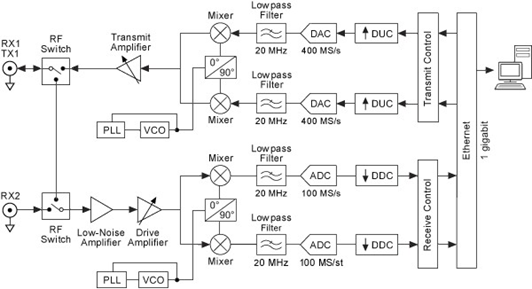
\includegraphics[width=.7\textwidth]{USRPblock.png}
                \caption{Τυπικό μπλοκ διάγραμμα ενός USRP}
                \label{fig:USRPblock}
            \end{figure}\\

            Στο εργαστήριό μας, θα χρησιμοποιήσουμε το υλικό USRP B200 και B210, 
            δείτε τα σχήματα (\ref{img:USRPfront}), (\ref{img:USRPback}) και 
            (\ref{img:USRPin}).
            Η σειρά B(us) USRP καλύπτει συχνότητες RF από 70 MHz έως 6 GHz, διαθέτει
            συνδεσιμότητα Spartan-6 FPGA και USB 3.0. 
            Αυτή η πλατφόρμα επιτρέπει τον πειραματισμό με ένα ευρύ φάσμα σημάτων,
            συμπεριλαμβανομένων FM και τηλεοπτικών εκπομπών, κινητής τηλεφωνίας, 
            Wi-Fi και άλλων. Το USRP B200 διαθέτει ένα κανάλι λήψης και ένα κανάλι μετάδοσης
            σε σχεδιασμό που τροφοδοτείται από δίαυλο. 
            Το USRP B210 επεκτείνει τις δυνατότητες του B200 προσφέροντας συνολικά δύο 
            κανάλια λήψης και δύο κανάλια μετάδοσης, ενσωματώνει ένα μεγαλύτερο FPGA,
            GPIO και περιλαμβάνει εξωτερικό τροφοδοτικό. Και οι δύο χρησιμοποιούν ένα RFIC
            αναλογικών συσκευών (AD9361) για να προσφέρουν μια οικονομικά αποδοτική 
            πλατφόρμα πειραματισμού RF και μπορούν να μεταδώσουν έως και 56 MHz στιγμιαίου
            εύρους ζώνης μέσω ενός διαύλου USB 3.0 υψηλού εύρους ζώνης σε επιλεγμένα 
            chipset USB 3.0 (με συμβατότητα προς τα πίσω με USB 2.0).

            \begin{figure}[h]
                \centering
                \begin{subfigure}{0.3\linewidth}
                    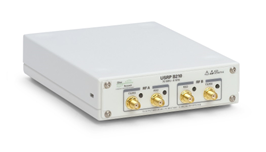
\includegraphics[width=\linewidth]{USRPback.png}
                    \caption{Back}
                    \label{img:USRPback}
                \end{subfigure}
                \begin{subfigure}{0.3\linewidth}
                    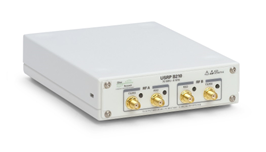
\includegraphics[width=\linewidth]{USRPback.png}
                    \caption{Front}
                    \label{img:USRPfront}
                \end{subfigure}
                \begin{subfigure}{0.3\linewidth}
                        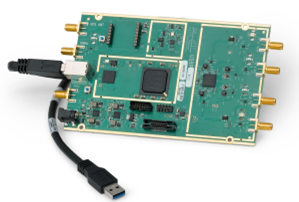
\includegraphics[width=\linewidth]{USRPin.png}
                        \caption{inside}
                        \label{img:USRPin}
                     \end{subfigure}
                \caption{Το FPGA υλισμικό του USRP}
                \label{fig:USRP}
            \end{figure}

        \subsection{\textsf{GNU Radio Software}}
            Το GNU Radio \footnote{wiki.gnuradio.org} \footnote{gnuradio.org} είναι μια ελεύθερη 
            και ανοιχτού κώδικα εργαλειοθήκη ανάπτυξης λογισμικού που παρέχει μπλοκ επεξεργασίας 
            σήματος για την υλοποίηση ραδιοφώνων λογισμικού. Μπορεί να χρησιμοποιηθεί με άμεσα 
            διαθέσιμο εξωτερικό υλικό RF χαμηλού κόστους για τη δημιουργία ραδιοφώνων που 
            καθορίζονται από λογισμικό ή χωρίς υλικό σε περιβάλλον προσομοίωσης. 
            Χρησιμοποιείται ευρέως από χομπίστες, σε ακαδημαϊκά και εμπορικά
            περιβάλλοντα για την υποστήριξη τόσο της έρευνας ασύρματων επικοινωνιών όσο και των
            πραγματικών ραδιοσυστημάτων. Το GNU Radio εκτελεί όλη την επεξεργασία σήματος. Μπορείτε
            να το χρησιμοποιήσετε για να γράψετε εφαρμογές, για να λάβετε δεδομένα από ψηφιακές ροές
            ή για να προωθήσετε δεδομένα σε ψηφιακές ροές, οι οποίες στη συνέχεια μεταδίδονται
            χρησιμοποιώντας υλικό. Το GNU Radio έχει φίλτρα, κωδικούς καναλιών, στοιχεία
            συγχρονισμού, ισοσταθμιστές, αποδι- αμορφωτές, αποκωδικοποιητές και πολλά άλλα στοιχεία
            (που ονομάζονται μπλοκ) τα οποία συνήθως βρίσκονται σε ραδιοσυστήματα. Το πιο σημαντικό,
            περιλαμβάνει μια μέθοδο σύνδεσης αυτών των μπλοκ και στη συνέχεια διαχειρίζεται τον
            τρόπο με τον οποίο τα δεδομένα μεταφέρονται από το ένα μπλοκ στο άλλο. Η επέκταση του
            GNU Radio είναι επίσης αρκετά εύκολη. Εάν βρείτε ένα συγκεκριμένο μπλοκ που λείπει,
            μπορείτε γρήγορα να το δημιουργήσετε και να το προσθέσετε γράφοντας κώδικα Python.
            Δεδομένου ότι το GNU Radio είναι λογισμικό, μπορεί να χειριστεί μόνο ψηφιακά δεδομένα.
            Συνήθως, μιγαδικά δείγματα βασικής ζώνης είναι ο τύπος δεδομένων εισόδου για δέκτες
            και ο τύπος δεδομένων εξόδου για πομπούς. Στη συνέχεια, χρησιμοποιείται αναλογικό υλικό
            για τη μετατόπιση του σήματος στην επιθυμητή κεντρική συχνότητα. Πέρα από αυτή την
            απαίτηση, οποιοσδήποτε τύπος δεδομένων μπορεί να περάσει από το ένα μπλοκ στο άλλο -
            είτε πρόκειται για bit, byte, διανύσματα, ριπές ή πιο σύνθετους τύπους δεδομένων. Οι
            εφαρμογές GNU Radio γράφονται κυρίως χρησιμοποιώντας τη γλώσσα προγραμματισμού Python,
            ενώ η παρεχόμενη, κρίσιμη για την απόδοση διαδρομή επεξεργασίας σήματος υλοποιείται σε
            C++ χρησιμοποιώντας επεκτάσεις κινητής υποδιαστολής επεξεργαστή, όπου είναι διαθέσιμες.
            Έτσι, ο προγραμματιστής είναι σε θέση να υλοποιήσει ραδιοσυστή- ματα υψηλής απόδοσης σε
            πραγμα- τικό χρόνο σε ένα απλό στη χρήση, γρήγορο περιβάλλον ανάπτυξης εφαρμογών. Το GNU
            Radio είναι ένα πλαίσιο που επιτρέπει στους χρήστες να σχεδιάζουν, να προσομοιώνουν και
            να αναπτύσσουν εξαιρετικά ικανά ραδιοσυστήματα πραγματικού κόσμου. Πρόκειται για ένα
            εξαιρετικά αρθρωτό πλαίσιο προσανατολισμένο στο "διάγραμμα ροής" που συνοδεύεται από μια
            ολοκληρωμένη βιβλιο- θήκη μπλοκ επεξεργασίας που μπορούν εύκολα να συνδυαστούν για να
            κάνουν πολύπλοκες εφαρμογές επεξεργασίας σήματος.

            \begin{figure}[h]
                \centering
                
\includegraphics[width=.9\textwidth]{gnuradio.png}
            \end{figure}
        
    \section{\textsf{I/Q Data}}
        Τα δεδομένα in-phase/quadrature (I/Q) είναι μια σύνθετη αναπαράσταση του μεταδιδόμενου
        σήματος, για το οποίο μπορούν όχι μόνο να δώσουν πληροφορίες σχετικά με το πλάτος των 
        σημάτων αλλά και τις πληροφορίες φάσης. Τα δεδομένα IQ μπορούν να αναπαρασταθούν ως δύο
        κανάλια δεδομένων που είναι ορθογώνια μεταξύ τους, όπως φαίνεται στο σχήμα (\ref{fig:I/Q}).

        \begin{figure}[h]
            \centering
            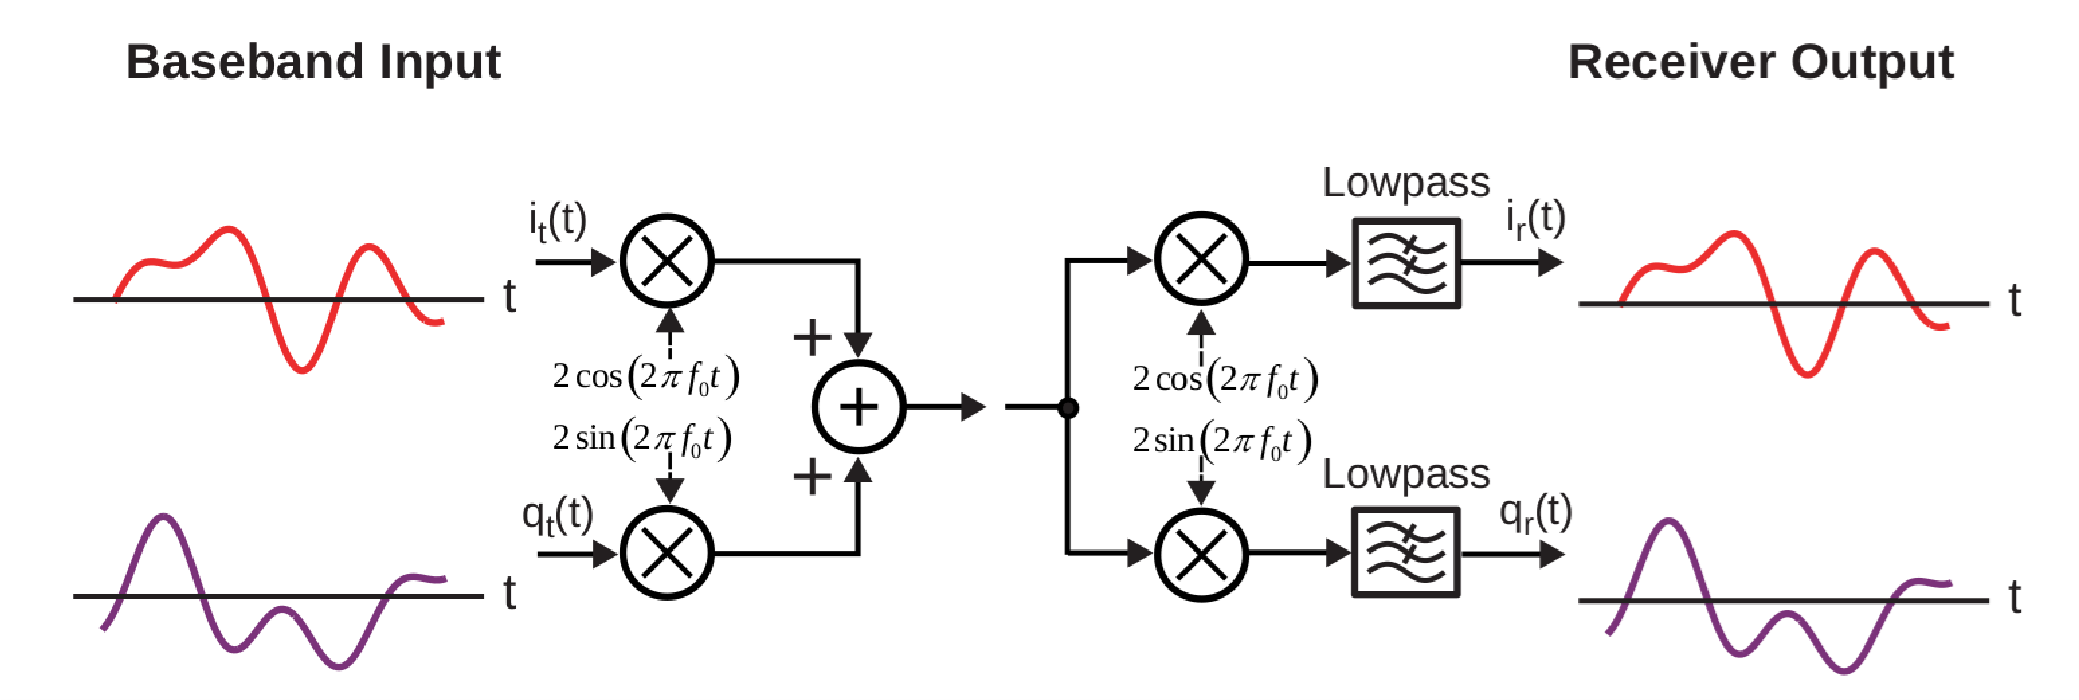
\includegraphics[width=.8\textwidth]{iq_diagram.png}
            \caption{Κανάλια In-Phase/Quadrature}
            \label{fig:I/Q}
        \end{figure}

        Τα δύο κανάλια στην πλευρά του πομπού μπορούν να γραφτούν ως εξής:\\


        \begin{equation}
            \label{eq:I/Q}
            \left\{\begin{array}{l}
                i(t) = i_t(t) \cos(2\pi f_0 t)\\
                q(t) = q_t(t) \sin(2\pi f_0 t)\\
            \end{array}\right.
        \end{equation}

        Και προσθέτοντας κατά μέλη: \begin{equation}\label{eq:I+Q}
            y(t) = i_t(t)\cos(2\pi f_0 t) + q_t(t)\sin(2\pi f_0 t)
        \end{equation}

        \newpage
        Από την μεριά του δέκτη τα δύο κανάλια μπορούν να ανακτηθούν χρησιμοποιώντας την
        τριγωνομετρική ταυτότητα γινομένου \rightarrow  άθροισμα. \footnote{
            $\cos(x) \times \cos(y) = \frac{1}{2} (\cos(x-y)+\cos(x+y))$,\qquad
            $\sin(x) \times \sin(y) = \frac{1}{2} (\cos(x-y)-\cos(x+y))$
            
            \quad
            $\sin(x) \times \cos(y) = \frac{1}{2} (\sin(x+y)+\sin(x-y))$,\qquad
            $\sin(x) \times \sin(y) = \frac{1}{2} (\sin(x+y)-\sin(x-y))$\\
        }

        \begin{align}
            i_r(t) &\quad = 2[i_t(t)\cos(2\pi f_0t) + q_t(t)\sin(2\pi f_0t)]\sin(2\pi f_0t)\nonumber\\
            &\quad = [i_t(t) + i_t(t)\cos(4\pi f_0t)]+[q_t(t)\sin(4\pi f_0t)+q_t(t)\sin(0)] \label{eq:Irec}\\
            &\quad = [i_t(t) + i_t(t)\cos(4\pi f_0t)]+[q_t(t)\sin(4\pi f_0t)]\nonumber            
        \end{align}

        \begin{align}
            q_r(t) &\quad = 2[i_t(t)\cos(2\pi f_0t) + q_t(t)\sin(2\pi f_0t)]\sin(2\pi f_0t)\nonumber\\
            &\quad = [i_t(t)\sin(4\pi f_0t)-i_t(t)\sin(0)] + [q_t(t)-q_t(t)\cos(4\pi f_0t)]\label{eq:Qrec}\\
            &\quad = [i_t(t)\sin(4\pi f_0t)] + [q_t(t)-q_t(t)\cos(4\pi f_0t)]\nonumber
        \end{align}


        Χρησιμοποιώντας ένα χαμηλοπερατό φίλτρο στον δέκτη τα κανάλια I\&Q μπορούν να ανακτηθούν.

    \section{\textsf{Διαδικασία Εργαστηρίου}}
        \subsection{\textsf{Δημιουργώντας ένα μπλόκ διάγραμμα}}

            Σε αυτήν την άσκηση θα παράξετε ένα συνημίτονο κύμα χρησιμοποιώντας το GNU Radio.

            \begin{itemize}
                \item Ανοίξτε ένα καινούριο διάγραμμα ροής
                \item Δύο πλαίσια θα βρίσκονται στο διάγραμμα ροής,
                    \begin{itemize}
                        \item "Επιλογές", το οποίο χρησιμοποιείται για τον ορισμό καθολικών παραμέτρων
                        για το διάγραμμα ροής.
                        \item "Μεταβλητή", το οποίο μπορείτε να του δώσετε ένα όνομα και να 
                        το χρησιμοποιήσετε στο διάγραμμα ροής σας (προεπιλεγμένη μεταβλητή είναι 
                        ο ρυθμός δειγματοληψίας\footnote{
                            Σκεφτείτε ότι ο ρυθμός δειγματοληψίας χρησιμοποιείται για τον υπολογισμό του 
                            διακριτού μεγέθους βημάτων από το ένα δείγμα στο επόμενο μέσα σε μια λειτουργία DSP.
                            Ο ρυθμός δειγματοληψίας αναφέρεται επίσης στο ρυθμό με τον οποίο τα δείγματα
                            διέρχονται από το διάγραμμα ροής. Εάν δεν υπάρχει έλεγχος ρυθμού, ρολόι υλικού ή
                            μηχανισμός στραγγαλισμού, τα δείγματα θα παραχθούν, θα περάσουν από το διάγραμμα 
                            ροής και θα καταναλωθούν όσο το δυνατόν γρηγορότερα (δηλαδή το διάγραμμα ροής θα
                            είναι δεσμευμένο από την CPU). Μόνο ένα μπλοκ που αντιπροσωπεύει κάποιο υποκείμενο
                            υλικό με το δικό του ρολόι (π.χ. USRP, κάρτα ήχου) ή το throttle μπλοκ, θα
                            χρησιμοποιήσει το "Sample Rate" για να ρυθμίσει αυτό το ρολόι υλικού και επομένως 
                            θα έχει ως αποτέλεσμα την εφαρμογή ελέγχου ρυθμού στα δείγματα στο διάγραμμα ροής.
                        })
                    \end{itemize}
                \item Ορίστε τις επιλογές δημιουργίας σε QT GUI.
                \item Προσθέστε ένα άλλο μπλοκ \textbf{\textit{μεταβλητής}}, 
                    ονομάστε το \textbf{freq} και ορίστε το σε \textbf{1000}.
                \item Προσθέστε μια \textbf{\textit{πηγή σήματος}} και ορίστε τον \textbf{τύπο εξόδου}
                σε \textbf{float}, \textbf{κυματομορφή} σε \textbf{συνημίτονο},\\
                \textbf{συχνότητα} σε \textbf{freq}, \textbf{πλάτος} σε \textbf{1} και τέλος 
                \textbf{μετατόπιση} σε \textbf{0}.
                \item Προσθέστε μια \textbf{\textit{Throttle}} και ορίστε το \textbf{Type} σε \textbf{Float}.
                \item Προσθέστε ένα \textbf{\textit{QT GUI Sink}} και ορίστε το \textbf{Type} σε \textbf{Float}
                και το \textbf{FFT Size} σε \textbf{1024}.
                \item Αλλάξτε τη συχνότητα της πηγής σήματος από 1k σε 2.5k, 5k, 16k και 100k 
                και παρατηρήστε το πεδίο χρόνου και συχνότητας.
                \item \textsf{Ερώτηση 1: Ποια είναι η διαφορά και γιατί;}
            \end{itemize}

            Τελικά, θα πρέπει να έχετε ένα διάγραμμα ροής όπως φαίνεται στο σχήμα (\ref{fig:grcSource}).
            \begin{figure}[ht]
                \centering
                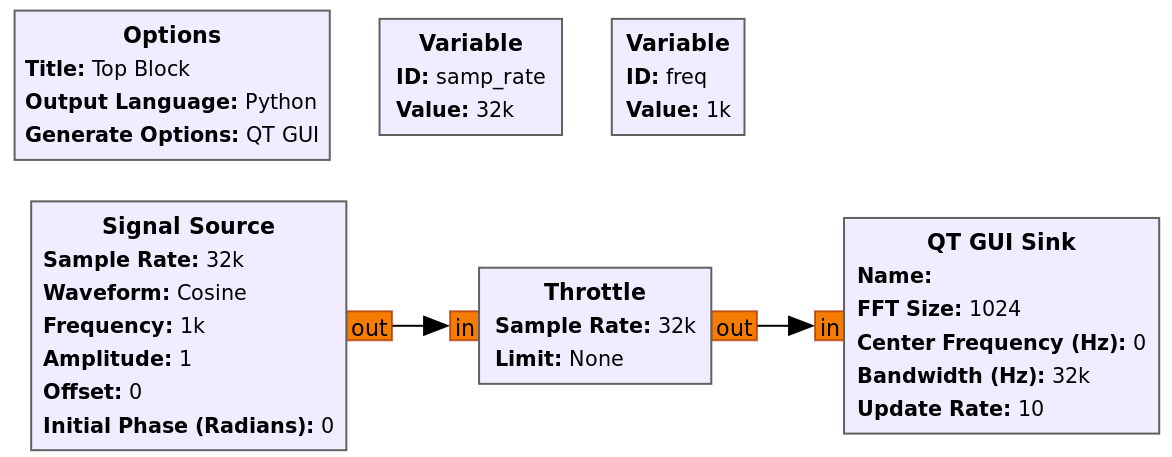
\includegraphics[width=.8\textwidth]{ex1_flow.png}
                \caption{Πηγή Σήματος GNU Radio}
                \label{fig:grcSource}
            \end{figure}

            Και όταν εκτελέσετε το διάγραμμα ροής θα λάβετε ένα αποτέλεσμα όπως φαίνεται στο 
            σχήμα (\ref{img:ex1}).
            \begin{figure}[h]
                \centering
                \begin{subfigure}{0.45\linewidth}
                    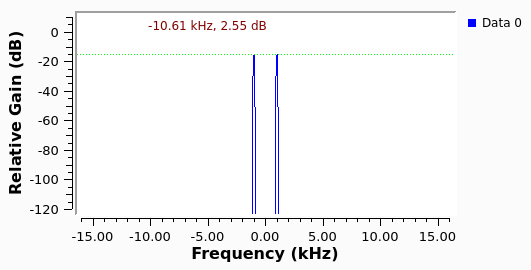
\includegraphics[width=\linewidth]{ex1_freq.png}
                    \caption{Πεδίο της Συχνότητας}
                    \label{img:ex1Freq}
                \end{subfigure}
                \begin{subfigure}{0.45\linewidth}
                    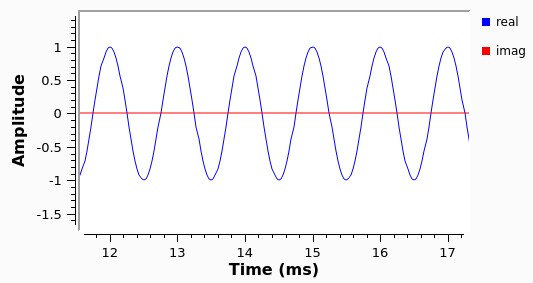
\includegraphics[width=\linewidth]{ex1_time.png}
                    \caption{Πεδίο του Χρόνου}
                    \label{img:ex1Time}
                \end{subfigure}

                \caption{Έξοδος του διαγράμματος ροής}
                \label{img:ex1}
            \end{figure}
        
        \subsection{\textsf{Μιγαδικό Σήμα με Θόρυβο}}

            Σε αυτή την άσκηση, θα δημιουργήσετε ένα μιγαδικό κύμα συνημιτόνου με θόρυβο.
            
            \begin{itemize}
                \item Ανοίξτε ένα καινούριο διάγραμμα ροής
                \item Ορίστε τις \textbf{\textit{επιλογές δημιουργίας}} σε \textbf{QT GUI}.
                \item Ορίστε τον \textbf{\textit{ρυθμό δειγματοληψίας}} σε \textbf{64000}.
                \item Προσθέστε ένα άλλο μπλοκ \textbf{\textit{μεταβλητής}}, 
                    ονομάστε το \textbf{freq} και ορίστε το σε \textbf{2000}.
                \item Προσθέστε μια \textbf{\textit{πηγή σήματος}} και ορίστε τον \textbf{τύπο εξόδου}
                σε \textbf{complex}, \textbf{κυματομορφή} σε \textbf{συνημίτονο},\\
                \textbf{συχνότητα} σε \textbf{freq}, \textbf{πλάτος} σε \textbf{1} και τέλος 
                \textbf{\textit{μετατόπιση}} σε \textbf{0}.
                \item Προσθέστε μια \textbf{\textit{πηγή θορύβου}} και ορίστε τον \textbf{τύπο εξόδου}
                    σε \textbf{μιγαδικούς} αριθμούς, τον \textbf{Τύπο θορύβου} σε \textbf{Gaussian} και το
                    \textbf{Πλάτος} σε \textbf{0.1}.
                \item Προσθέστε ένα μπλόκ \textbf{πρόσθεσης}.
                \item Προσθέστε ένα \textbf{\textit{Throttle}} και ορίστε το \textbf{Type} σε \textbf{Complex}.
                \item Προσθέστε ένα \textbf{\textit{QT GUI Sink}} και ορίστε το \textbf{Type} σε \textbf{Complex}.
                και το \textbf{FFT Size} σε \textbf{1024}.
                \item \textsf{Ερώτηση 2: Πόσες κορυφές συχνότητας μπορείτε να δείτε και γιατί;}
                \item \textsf{Ερώτηση 3: Πώς μπορείτε να μετριάσετε το φαινόμενο του θορύβου;}
            \end{itemize}

            Τελικά, θα πρέπει να έχετε ένα διάγραμμα ροής όπως φαίνεται στο σχήμα (\ref{fig:grcSourceWGN}).
            \begin{figure}[h]
                \centering
                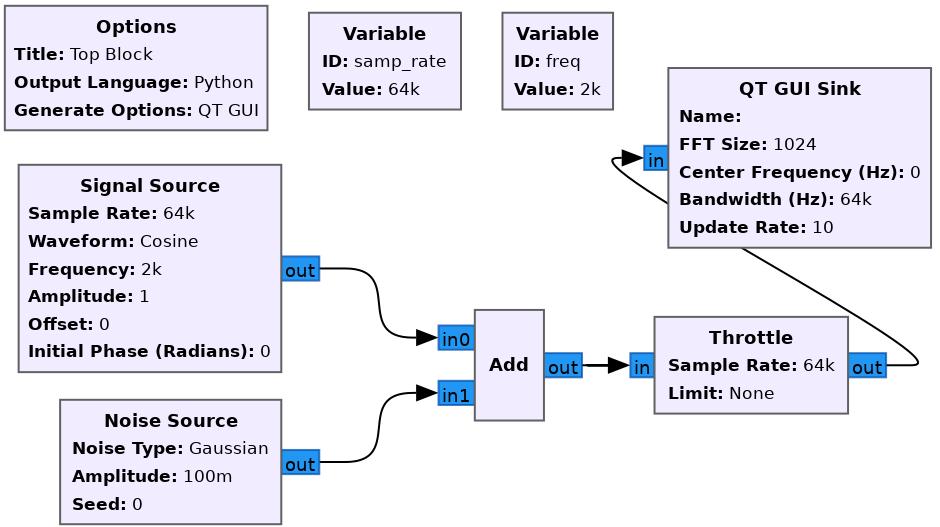
\includegraphics[width=.8\textwidth]{ex2_flow.png}
                \caption{Σύνθετο σήμα με θόρυβο}
                \label{fig:grcSourceWGN}
            \end{figure}

            Και όταν εκτελέσετε το διάγραμμα ροής θα λάβετε ένα αποτέλεσμα όπως φαίνεται στο 
            σχήμα (\ref{img:ex2}).
            \begin{figure}[h]
                \centering
                \begin{subfigure}{0.45\linewidth}
                    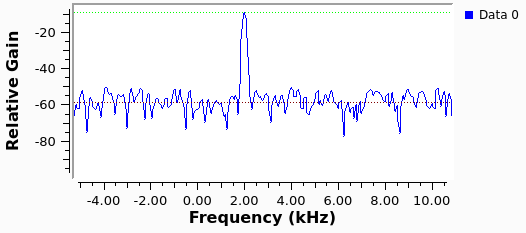
\includegraphics[width=\linewidth]{ex2_freq.png}
                    \caption{Πεδίο της Συχνότητας}
                    \label{img:ex2Freq}
                \end{subfigure}
                \begin{subfigure}{0.45\linewidth}
                    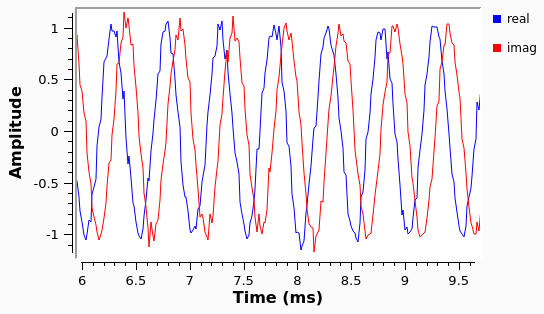
\includegraphics[width=\linewidth]{ex2_time.png}
                    \caption{Πεδίο του Χρόνου}
                    \label{img:ex2Time}
                \end{subfigure}

                \caption{Έξοδος του διαγράμματος ροής}
                \label{img:ex2}
            \end{figure}

        \subsection{\textsf{Συνδέοντας το USRP}}

            Σε αυτή την άσκηση θα μεταδώσετε και θα λάβετε ένα σύνθετο κύμα συνημιτόνου χρησιμοποιώντας το USRP.

            \begin{itemize}
                \item Ανοίξτε ένα καινούριο διάγραμμα ροής
                \item Ορίστε τις \textbf{\textit{επιλογές δημιουργίας}} σε \textbf{QT GUI}.
                \item Ορίστε τον \textbf{\textit{ρυθμό δειγματοληψίας}} σε \textbf{1e6}.
                \item Προσθέστε ένα άλλο μπλοκ \textbf{\textit{μεταβλητής}}, 
                    ονομάστε το \textbf{freq} και ορίστε το σε \textbf{20e3}.
                \item Προσθέστε ένα άλλο μπλοκ \textbf{\textit{μεταβλητής}}, 
                    ονομάστε το \textbf{carrier\_freq} και ορίστε το σε \textbf{1e9}.
                \item Προσθέστε μια \textbf{\textit{πηγή σήματος}} και ορίστε τον \textbf{τύπο εξόδου}
                    σε \textbf{complex}, \textbf{κυματομορφή} σε \textbf{συνημίτονο},\\
                    \textbf{συχνότητα} σε \textbf{freq}, \textbf{πλάτος} σε \textbf{1} και τέλος 
                \textbf{\textit{μετατόπιση}} σε \textbf{0}.
                \item Προσθέστε ένα \textbf{\textit{UHD: USRP Sink}} και ορίστε τον \textbf{τύπο εισόδου}
                    σε \textbf{complex float32}, την \textbf{Κεντρική Συχνότητα} σε \textbf{carrier\_freq} και την
                    \textbf{Τιμή Απολαβής} σε \textbf{1}.
                \item Προσθέστε ένα \textbf{\textit{UHD: USRP Source}} και ορίστε τον \textbf{τύπο εξόδου}
                    σε \textbf{complex float32}, την \textbf{Κεντρική Συχνότητα} σε \textbf{carrier\_freq} και την
                    \textbf{Τιμή Απολαβής} σε \textbf{0}.
                \item Προσθέστε ένα \textbf{\textit{QT GUI Sink}} και ορίστε το \textbf{Type} σε \textbf{Complex}
                και το \textbf{FFT Size} σε \textbf{1024}.
                \item Προσθέστε ένα φίλτρο ώστε να ανακτήσετε το σωστό σήμα με λιγότερο θόρυβο.
                \item \textsf{Ερώτηση 4: Ποιο φίλτρο χρησιμοποιείτε και ποιες είναι οι παράμετροι που θα επιλέξετε;}
            \end{itemize}

            Στο τέλος θα πρέπει να έχετε ένα διάγραμμα ροής όπως φαίνεται στην εικόνα (\ref{img:USRPsrc}).
            \begin{figure}[h]
                \centering
                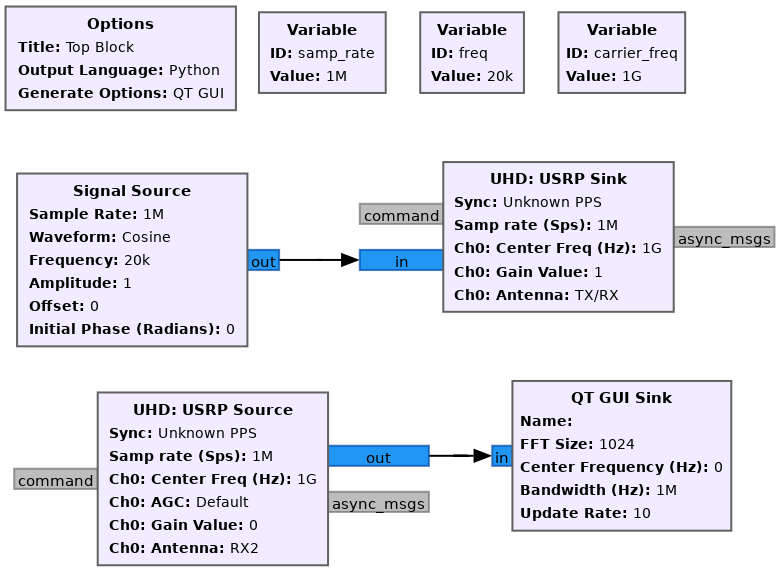
\includegraphics[width=.8\textwidth]{ex3_flow.png}
                \caption{USRP ως Πηγή Σήματος}
                \label{img:USRPsrc}
            \end{figure}

\end{document}